\chapter{Segmentazione Delle Facciate}
\label{sez:Segmentazione}
In questo capitolo si descriverà come è stato affrontato il problema dell'estrazione delle facciate degli edifici a partire da una grande point cloud che rappresentava una vasta area. 
Per questo scopo è stata utilizata Point Cloud Library.

\section{PCL (Point Cloud Library)}
\label{sez:PCL}

\textbf{P}oint \textbf{C}loud \textbf{L}ibrary \cite{pcl} è un progetto open source per processare point cloud. Esso include e implementa un grande numero di algoritmi che consentono di filtrare, manipolare, segmentare ed estrarre features da point cloud. PCL è un progetto modulare, diviso in tante librerie che possono essere usate e compilate separatemente.
L'albero delle librerie è il seguente:

\begin{figure}[ht!]
    \centering
    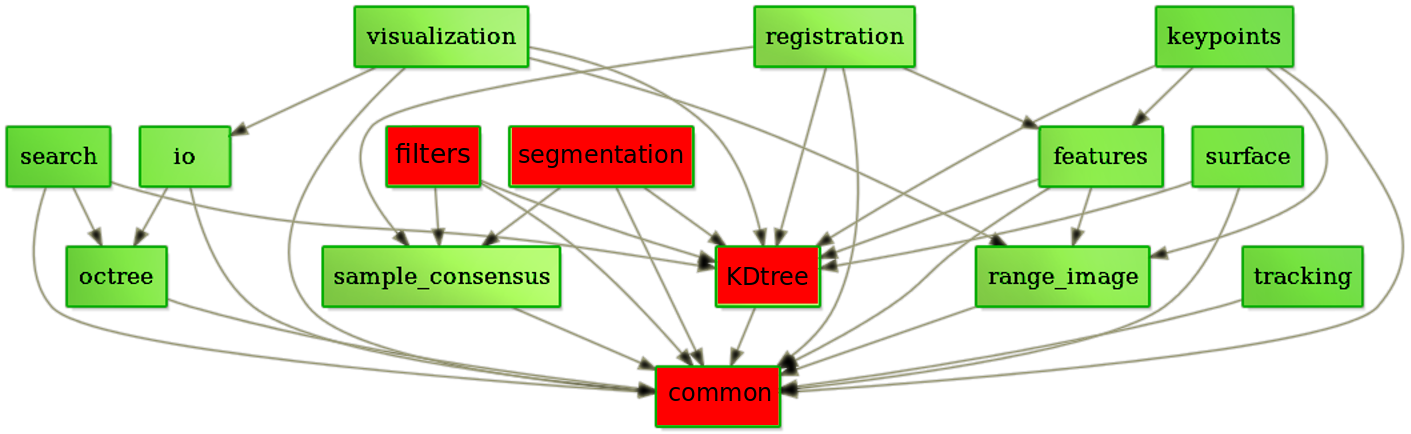
\includegraphics[width=0.7\textwidth]{Immagini/pcl_dependency_graph2.png}
    \caption{Grafo delle librerie di PCL, in rosso le librerie utilizzate}
    \label{fig:PCLGraph}
\end{figure}

In particolare sono state utilizzate le librerie inerenti al filtraggio, alla segmentazione e all'utilizzo di alberi KDTree.

PCL è stata utilizzata per la segmentazione delle facciate degli edifici ovvero per andare ad estrarre le singole facciate a partire dalla point cloud della mappa.\\
Si andrà ora a descrivere nel dettaglio il procedimento di segmentazione attuato.

\section{Filtraggio in altezza}
Per riuscire a trovare più facilmente le facciate si è deciso di effettuare un filtraggio della point cloud in modo da eliminare punti superflui come quelli del piano stradale o dei marciapiedi e ridurre così i tempi di calcolo.\newline
Si è deciso di optare per un filtro sulle altezze strutturato nel seguente modo:
\begin{equation}
    P_{cf}(x,y,z) = \{P(x,y,z) \in PC : h_{min} < z < h_{max}\}
    \label{eq:Filte}
\end{equation}
Nel nostro caso si è deciso per filtrare tutti i punti con un'altezza inferiore ai 15 cm, considerandoli come manto stradale, e tutti i punti con un'altezza superiore ai 50m.\newline

La condizione si è tradotta nel seguente frammento di codice:
\begin{lstlisting}[caption={Filtraggio della pointcloud},captionpos=b,language=cpp]
  pcl::PassThrough<pcl::PointXYZ> pass;
  pass.setInputCloud (cloud);
  pass.setFilterFieldName ("z");
  pass.setFilterLimits (0.15,50);
  pass.filter (*cloud_filtered);
\end{lstlisting}

Il risultato dell'operazione di filtraggio è il seguente:

\begin{figure}[H]
\centering
       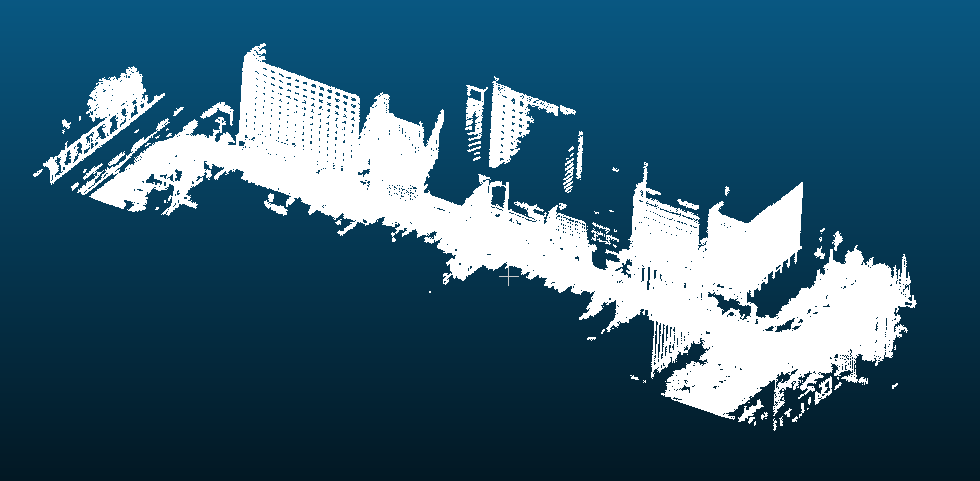
\includegraphics[width=0.9\textwidth]{Immagini/PC.png}
       \caption{Point cloud prima del filtraggio}
       \label{fig:PC} 
\end{figure}
\begin{figure}[H]
\centering
       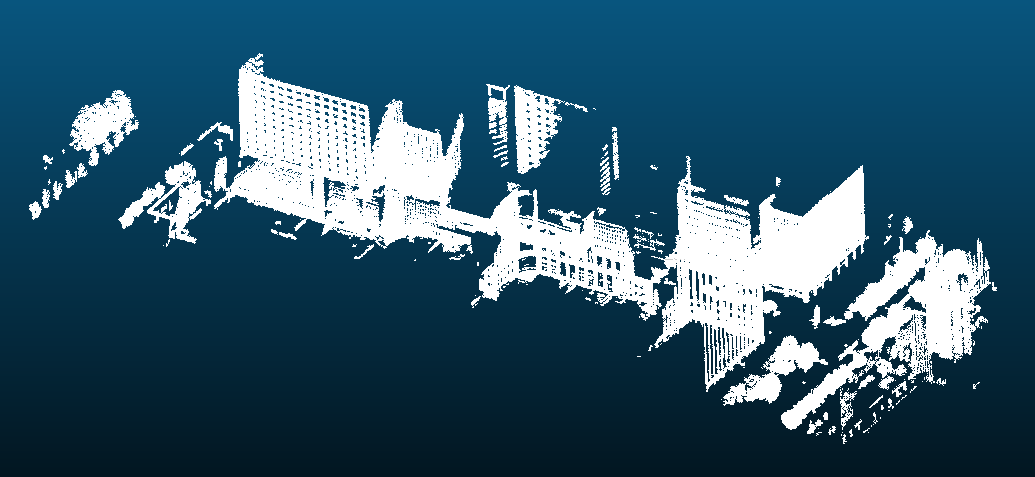
\includegraphics[width=0.9\textwidth]{Immagini/PCFiltered.png}
       \caption{Point cloud  dopo il filtraggio}
       \label{fig:PCfiltered}
\end{figure}
Come si può notare sono stati rimossi tutti i punti relativi al manto stradale e ai marciapiedi.

\section{Differenza di Normali}
E' stata successivamente applicata una segmentazione attraverso l'utilizzo della differenza di normali \cite{don}.
\\L'operatore \textit{DoN} si basa sull'uso delle normali stimate dalle superfici appartenenti ad una point cloud non organizzata ovvero in cui i punti non hanno un particolare ordine.
L'operatore è definito come:

\begin{equation}
    \Delta\hat{n}(p,r_s,r_l) = \frac{\hat{n}(p,r_s)-\hat{n}(p,r_l)}{2}
    \label{eq:DoNOperator}
\end{equation}

Dove $$r_s \:e\: r_l$$ sono rispettivamente i raggi di supporto della normale. \newline
La motivazione principale che sta alla base dell'uso di questo operatore è data dall'osservazione del fatto che, dato un raggio di supporto, la normale viene stimata trovando il piano tangente alla componente principale dell'intorno dei punti appartenenti al raggio stesso. \newline
In questo modo la normale riflette la geometria della superficie sottostante al punto in base alle dimensioni del raggio di supporto. Cambiando il raggio di supporto la direzione della normale cambia in base alla geometria della superficie sottostante (\ref{fig:DoNsurface}).
\newline
Inoltre le normali sono caratteristiche che, all'interno di una point cloud, risultano poco affette da rumore per la loro natura. 
Esse infatti vengono sempre stimate tramite un raggio di supporto, o un numero prefissato di vicini, caratteristica che premette di ridurre il peso di eventuali punti rumorosi.

\begin{figure}[h!]
    \centering
    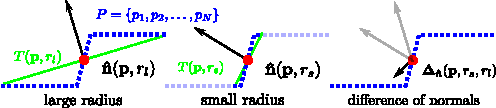
\includegraphics[width=0.8\textwidth]{Immagini/don_scalenormals.pdf}
    \caption{Effetti dei differenti raggi per la stima di una superficie}
    \label{fig:DoNsurface}
\end{figure}

L'operazione può facilmente essere svolta con \hyperref[sez:PCL]{\textbf{PCL}}:

\begin{lstlisting}[caption={Applicazione della DoN},captionpos=b,language=cpp]
    pcl::NormalEstimationOMP<PointXYZ, PointNormal> ne;
    ne.setInputCloud (cloud);
    ne.setSearchMethod (tree);
    ne.setViewPoint (std::numeric_limits<float>::max (),     std::numeric_limits<float>::max (), std::numeric_limits<float>::max ());
    pcl::PointCloud<PointNormal>::Ptr normals_small_scale (new   pcl::PointCloud<PointNormal>);
    ne.setRadiusSearch (scale1);
    ne.compute (*normals_small_scale);
    pcl::PointCloud<PointNormal>::Ptr normals_large_scale (new     pcl::PointCloud<PointNormal>);
    ne.setRadiusSearch (scale2);
    ne.compute (*normals_large_scale);
    pcl::DifferenceOfNormalsEstimation<PointXYZ, PointNormal, 
    PointNormal> don;
    don.setInputCloud (cloud);
    don.setNormalScaleLarge (normals_large_scale);
    don.setNormalScaleSmall (normals_small_scale);
\end{lstlisting}
\vspace{1cm} 

Come è stato evidenziato da dati sperimentali \cite{don} sono stati scelti come raggi 0.8 e 8.0. \newline
Il risultato dell'applicazione della DoN sulla pointcloud è il seguente: 

\begin{figure}[H]
    \centering
    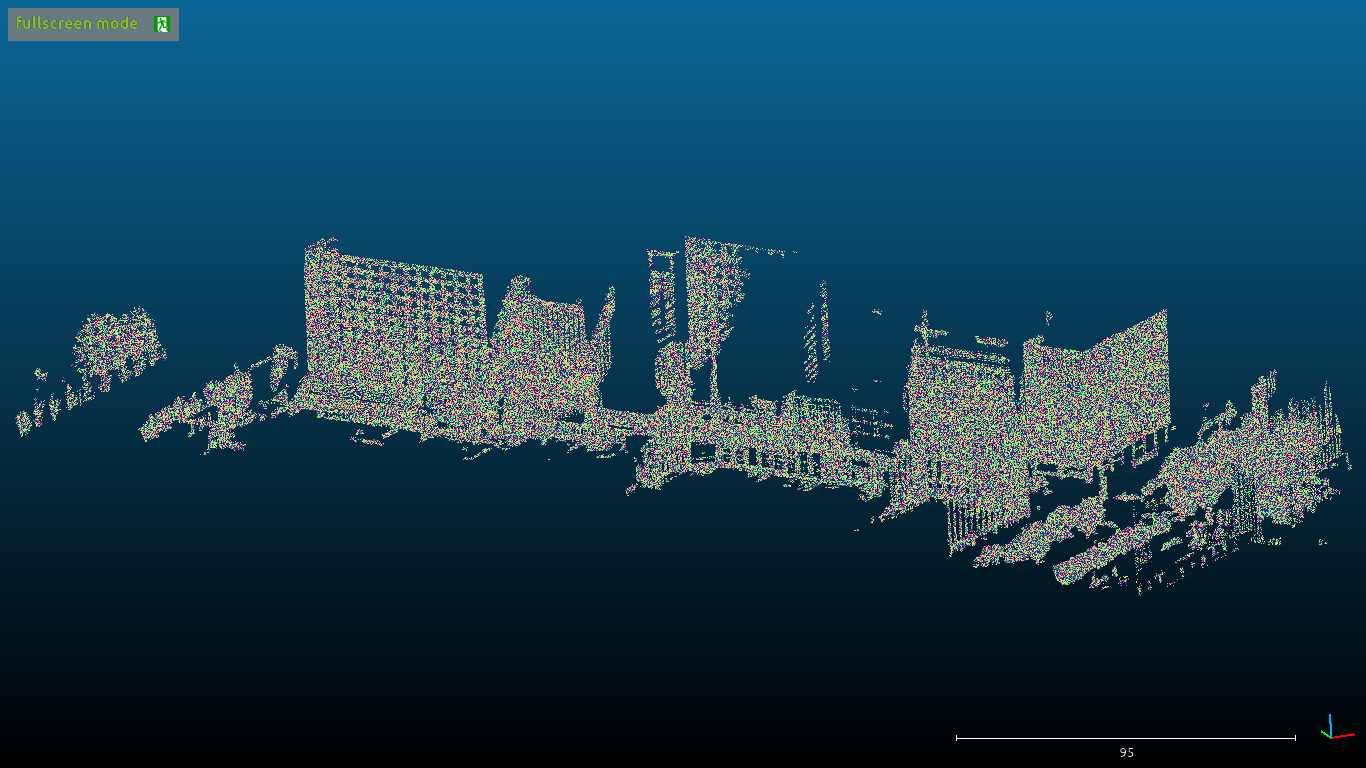
\includegraphics[width=0.7\textwidth]{Immagini/DoN.png}
    \caption{E' possibile vedere le diverse normali calcolate sulla point cloud}
    \label{fig:DoN}
\end{figure}

Si è passato poi al filtraggio della nuvola di punti generata dopo l'applicazione dell'operatore DoN (\ref{eq:DoNOperator}) in modo da discriminare i punti appartenenti ad una facciata. \newline
Dal momento che il risultato dell'applicazione dell'operatore DoN (\ref{eq:DoNOperator}) è un vettore, si è scomposto nelle sue 3 componenti:

\begin{equation}
    \begin{cases}
    \Delta\hat{n}(p,r_s,r_l)_x \in (-1, 1) \\
    \Delta\hat{n}(p,r_s,r_l)_y \in (-1, 1) \\
    \Delta\hat{n}(p,r_s,r_l)_z \in (-1, 1) \\
    \end{cases}
\end{equation}{}

Si è poi evidenziato empiricamente che il miglior modo per filtrare i punti appartenenti alla stessa facciata è quello di prendere punti con $\Delta\hat{n}(p,r_s,r_l)_z$ e $\Delta\hat{n}(p,r_s,r_l)_y$ molto grandi e con $\Delta\hat{n}(p,r_s,r_l)_x$ piccola. Per tanto si è impostato un filtro che filtrasse la nuvola di punti rispettando le condizioni sopra imposte. Si è ottenuta quindi la seguente condizione:
\begin{lstlisting}[caption={Filtraggio della pointcloud dopo l'applicazione dell' operatore DoN},captionpos=b,language=cpp]
    pcl::ConditionOr<PointNormal>::Ptr range_cond (
    new pcl::ConditionOr<PointNormal> ()
    );
  range_cond->addComparison (pcl::FieldComparison<PointNormal>::ConstPtr (
                               new pcl::FieldComparison<PointNormal> ("normal_z", pcl::ComparisonOps::GT, z_normthreshold))
                             );
  range_cond->addComparison (pcl::FieldComparison<PointNormal>::ConstPtr (
                               new pcl::FieldComparison<PointNormal> ("normal_y", pcl::ComparisonOps::GT, y_normthreshold))
                             );

     pcl::ConditionAnd<PointNormal>::Ptr range1_cond (
    new pcl::ConditionAnd<PointNormal> ()
    );        
    range1_cond -> addComparison (pcl::FieldComparison<PointNormal>::ConstPtr (
                               new pcl::FieldComparison<PointNormal> ("normal_x", pcl::ComparisonOps::LT, x_normthreshold))
                             );        
    range1_cond -> addCondition(range_cond);
    
    pcl::ConditionalRemoval<PointNormal> condrem;
    condrem.setCondition (range1_cond);
    condrem.setInputCloud (doncloud);
    pcl::PointCloud<PointNormal>::Ptr doncloud_filtered (new pcl::PointCloud<PointNormal>);
    
    condrem.filter (*doncloud_filtered);
    doncloud = doncloud_filtered;
\end{lstlisting}
Il risultato ottenuto è il seguente:
\begin{figure}[H]
    \centering
    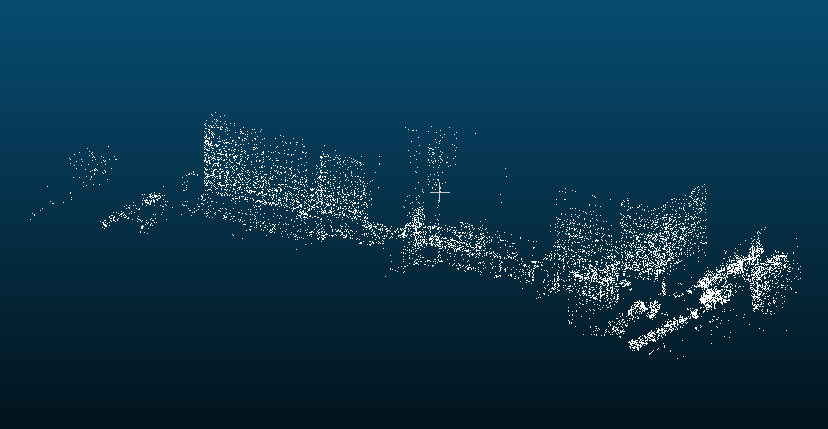
\includegraphics[width=0.9\textwidth]{Immagini/Don_Filtered.png}
    \caption{E' possibile notare come gli alberi e altre strutture non appartenenti alle facciate degli edifici siano state eliminate}
    \label{fig:DoNfiltered}
\end{figure}
\newpage
\section{Clustering}

L'operazione finale che è stata applicata per poter ottenere le facciate dei singoli edifici è stata quella del clustering. \newline
E' stato scelto di applicare un algoritmo di clustering basato sulla distanza euclidea tra i punti nello spazio \cite{RusuDoctoralDissertation}.
L'algoritmo procede nel modo seguente:

\begin{algorithm}[H]
\begin{algorithmic}{}
    \State $C = \emptyset, P, Q$
    \For{$p_i \in P$}
        \State $Q \leftarrow p_i$
        \ForAll{$p_i \in Q$}
            \For{$r < d_{th}$}
                \State $P^i_k \leftarrow p_i$
            \EndFor
            \For{$p^i_k \in P^i_k$}
                \If {$p^i_k \notin Q$}
                    \State $Q \leftarrow p^i_k$
                \EndIf
            \EndFor
        \EndFor
        \State $C \leftarrow Q$
        \State $Q = \emptyset$
    \EndFor
    \State \Return $C$
\end{algorithmic}
 \caption{Funzionamento dell'algoritmo di clustering}
 \label{alg:Clustering}
\end{algorithm}

Dove $P$ è la point cloud da clusterizzare, $C$ è una lista contenente i cluster e $Q$ è una coda che contiene i vari punti da processare, $d_{th}$ indica la distanza massima a cui cercare da ciascun punto ed $r$ è il raggio della sfera costruita a partire da un punto $p_i$.

L'algoritmo va a cercare tutti i punti vicini ad un altro all'interno di un raggio prestabilito e li inserisce dentro lo stesso cluster, il funzionamento è similare a quello di k-Nearest Neighbour \cite{knn}.
\textbf{PCL} consente di implementare facilmente questo tipo di clustering attraverso la classe \textit{pcl::EuclideanClusterExtraction class} contenuta all'interno di \hyperref[sez:PCL]{\textbf{PCL}}, questa classe consente inoltre di specificare la dimensione minima e massima di un cluster. Attraverso varie prove si è ottenuto che le dimensioni ideali siano rispettivamente di 300 e di 1,000,000 di punti.
In codice ciò viene tradotto come:

\begin{lstlisting}[caption={Clustering usando PCL},captionpos=b,language=cpp]
  pcl::search::KdTree<PointNormal>::Ptr segtree (new pcl::search::KdTree<PointNormal>);
  segtree->setInputCloud (doncloud);
  std::vector<pcl::PointIndices> cluster_indices;
  pcl::EuclideanClusterExtraction<PointNormal> ec;
  ec.setClusterTolerance (segradius);
  ec.setMinClusterSize (300);
  ec.setMaxClusterSize (1000000);
  ec.setSearchMethod (segtree);
  ec.setInputCloud (doncloud);
  ec.extract (cluster_indices);

  int j = 0;
  for (std::vector<pcl::PointIndices>::const_iterator it = cluster_indices.begin (); it != cluster_indices.end (); ++it, j++)
  {
    pcl::PointCloud<PointNormal>::Ptr cloud_cluster_don (new pcl::PointCloud<PointNormal>);
    for (std::vector<int>::const_iterator pit = it->indices.begin (); pit != it->indices.end (); ++pit)
    {
      cloud_cluster_don->points.push_back (doncloud->points[*pit]);
    }
    cloud_cluster_don->width = int (cloud_cluster_don->points.size ());
    cloud_cluster_don->height = 1;
    cloud_cluster_don->is_dense = true;

    stringstream ss;
    ss << "don_cluster_" << j << ".pcd";
    writer.write<pcl::PointNormal> (ss.str (), *cloud_cluster_don, false);
  }
\end{lstlisting}{}

Abbiamo quindi diversi cluster ciascuno corrispondente ad una diversa facciata di ogni edificio.

\begin{figure}[H]
    \centering
    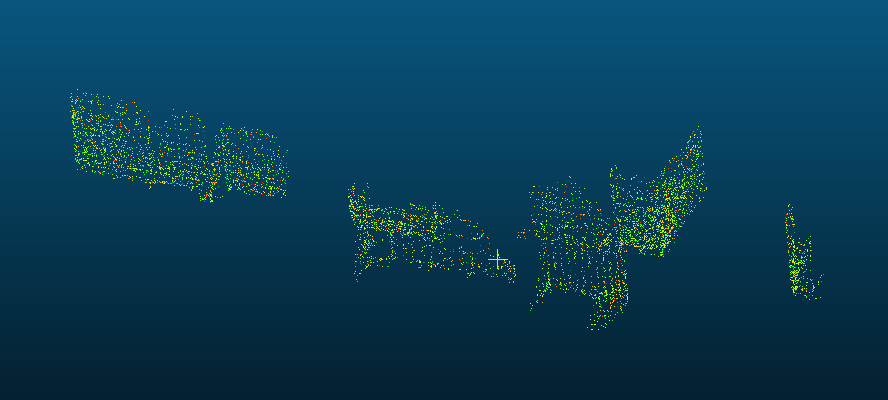
\includegraphics[width=0.7\textwidth]{Immagini/clusters.png}
    \caption{E' possibile vedere i cluster ottenuti rappresentanti le varie facciate degli edifici}
    \label{fig:clusters}
\end{figure}

I Cluster ottenuti verranno poi utilizzati per l'inserimento all'interno delle mappe di \hyperref[sez:OSM]{\textbf{OpenStreetMaps}}.